\chapter{Diseño e Implementación}

En este capítulo mostraremos los detalles del diseño y la implementacion de diferentes partes del proyecto.

\section{Gramáticas y frases}

La parte de la generación automática de frases y definición de gramáticas es la más relevante del proyecto y la que la diferencia del resto de juegos de similares caracteríticas. Por ello consideramos esencial mostrar su funcionamiento.

\begin{figure}
    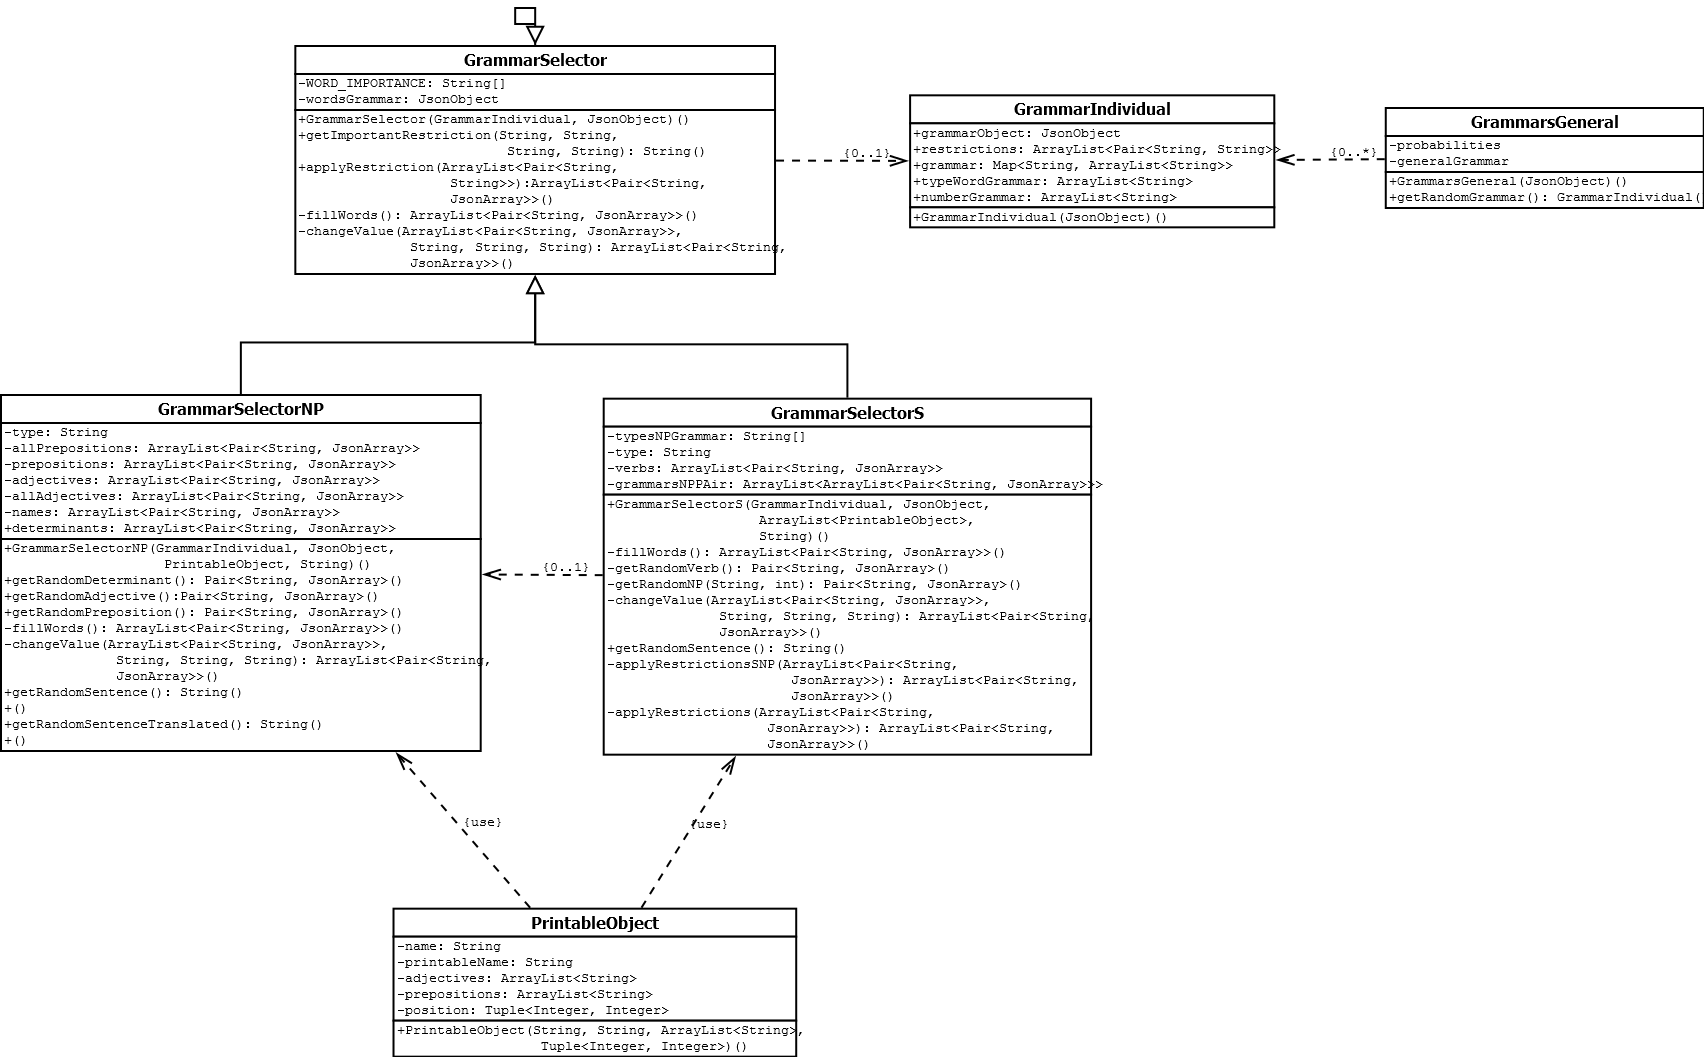
\includegraphics[width=\textwidth,height=\textheight,keepaspectratio,angle=90]{./img/grammarDiagram.png}
  \caption{Diagrama de clases de las gramáticas}
  \label{fig:clasesgramaticas}
\end{figure}

Tal y como se muestra en la figura ~\ref{clasesgramaticas}, la parte esencial de esta sección consta de seis clases, cuyo funcionamiento detallarremos a continuación.

\subsection{Explicación general del funcionamiento}

Tenemos dos clases (GrammarSelectorS y GrammarSelectorNP) que se encargan de generar las frases de manera aleatoria en base al nombre o nombres sobre los que queremos obtener dicha frase. La clase GrammarSelectorNP crea sintagmas nominales mientras que GrammarSelectorS crea frases usando dichos sintagmas nominales. Ambas usan diccionarios y gramáticas en un idioma en concreto especificado en el archivo de configuración \textit{language.properties}:

\begin{verbatim}
language=EN
\end{verbatim}

Parte de la dificultad de generar estas frases está en que todos los elementos de la misma deben de coincidir en base a las restricciones del propio idioma. Por ejemplo, los nombres, verbos y determinantes de una frase en español deben de coincidir en género y número. Este tipo de restricciones vienen dadas en las gramáticas que están especificadas en archivos JSON y que se comentarán más adelante.

Una vez detectemos que dos de las palabras no coinciden, cambiaremos la que tenga menor relevancia por la contraria dependiendo del tipo que sea (género o número):

\begin{lstlisting}[language=java]

if (toChange.equals(value1)) {
    changeToValue = JSONParsing.getElement(restrictions1, type + "opposite");
    typeChangeToValue = typeFirstRestriction; 
     
} else {
    changeToValue = JSONParsing.getElement(restrictions2, type + "opposite");
    typeChangeToValue = typeSecondRestriction;
}
this.changeValue(sentenceArray, toChange, changeToValue, typeChangeToValue);

\end{lstlisting}

De esta manera, siempre que haya una discordancia entre algunas de las palabras de una frase, iteraremos entre toda ella buscando una solución hasta que la frase sea coherente.

La clase GeneralGrammar, por su parte, obtiene la información de varias gramáticas (que es como vienen dadas en el fichero, dado que para describir una misma situación puede haber varias gramáticas que funcionen de la misma forma) y dispone de una función que devuelve una gramática individual (de la clase GrammarIndividual), que es la que usaremos a la hora de generar la frase en sí. Es decir, cuando queremos generar una frase de una gramática en concreto (por ejemplo cuando un personaje ataca a otro), seleccionaremos una de estas gramáticas al azar de todas las que estén disponibles en el idioma que tenemos (esto lo realiza la clase GrammarsGeneral) y luego usamos esa gramática en particular con GrammarIndividual.  De esta forma no siempre usamos la misma gramática y dependerá de la seleccionada aleatoriamente en GrammarsGeneral.

La clase PrintableObject es una superclase abstracta de la que heredan todos los objetos que pueden ser representados en el juego. Esta clase se encarga de obligar que dichos objetos tengan ciertas variables como el nombre o la capacidad de traducir su nombre a diferentes idiomas, así como una función que devuelve la posición en la que se encuentra en base al usuario (usado a la hora de describir lo que hay alrededor de un personaje).

Cabe destacar que estas gramáticas, al igual que los diccionarios usados para cada uno de los idiomas, se obtienen en base a ficheros JSON dados.

\subsection{\textit{Input} de gramáticas y diccionario}

Tal y como hemos mencionado anteriormente, tanto las gramáticas como los diccionarios son archivos JSON que el usuario puede cambiar y que afectará al resultado de las frases generadas por el juego.

Para las gramáticas tenemos dos archivos por idioma. Uno de ellos son las gramáticas con las que creamos sintagmas nominales, mientras que las otras creamos frases usando, en su mayor parte, estos sintagmas nominales.

\subsubsection{Gramáticas: Sintagmas nominales}

Ejemplo de gramáticas de sigtagma nominal en inglés:

\begin{lstlisting}[style=json]
"DETADJN": {
    "GM_1": {
        "S": 
            [
            {"DET_1": ""}, 
            {"ADJ_1": ""}, 
            {"N_1": ""}
        ],
        "restrictions": [
            {"DET_1.num": "N_1.num"},
            {"N_1.num": "ADJ_1.num"}
        ]
    }
}
\end{lstlisting}

En estas gramáticas especificamos, primero, el nombre de la gramática (en este caso, DETADJN). Este nombre es usado por el programa y ayudará al usuario a entender el tipo de gramática o grupo de gramáticas que son.

El siguiente nombre es el nombre de la gramática en particular. No es usado en el programa, pero su uso es necesario para poder definir varias gramáticas sobre el mismo árbol (si queremos varias gramáticas de tipo DETADJN, necesitaremos que se especifiquen el nombre de cada una de ellas).

Luego viene el contenido relevante. Primero nos encontramos con \textit{S}, que es donde encontraremos la definición de la gramática en sí; y luego \textit{restrictions} que, como su nombre indica, es especificaremos las restricciones.

En la parte de la gramática tenemos, en este caso, \textit{DET\_1}, que es el primer determinante (y único) de la gramática, \textit{ADJ\_1}, el primer y único adjetivo que tiene dicha gramática y \textit{N\_1}, que es el nombre o sustantivo.
En las restricciones detallaremos las partes de la gramática que tienen que coincidir. En esta gramática solamente tenemos que el determinante, nombre y adjetivo tienen que ser iguales en número. Es decir, que ``the red swords'' no sería generada, sino que generaría ``the red sword''.

Este es un ejemplo en inglés, cuyas restricciones son más sencillas que en otros idiomas como el español o el gallego, donde el nombres, determinante y adjetivo no solamente tiene que coincidir número, pero también en género. Por este motivo, para generar el mismo tipo de gramática para estos idiomas, necesitaremos hacer lo siguiente:

\begin{lstlisting}[style=json]
"DETADJN": {
    "GM_1": {
        "S": 
            [
            {"DET_1": ""},
            {"N_1": ""},
            {"ADJ_1": ""}
        ],
        "restrictions": [
            {"DET_1.num": "N_1.num"},
            {"N_1.num": "ADJ_1.num"},
            {"DET_1.gen": "N_1.gen"},
            {"N_1.gen": "ADJ_1.gen"}
        ]
    }
}
\end{lstlisting}

Nótese que no solamente hemos añadido el género a las restricciones (para que no podamos generar frases como ``la espada rojo'' o ``el espada roja''), pero también hemos cambiado el orden del nombre y adjetivo para que se adapten a ambos idiomas. 

A la hora de cambiar las palabras disponemos de un array donde ordenamos las palabras por importancia. Un sustantivo es más importante que un determinante, por lo que si una de las restricciones no se cumple por culpa de algunos de estos dos elementos, el determinante será en que cambiará para adaptarse al nombre.

De esta manera podemos adaptar gramáticas a idiomas diferentes de una forma muy fácil y sin necesidad de tocar nada de código.

\subsubsection{Gramáticas: Frases}

Las gramáticas para la generación de frases también usa las gramáticas de sintagma nominal: 

\begin{lstlisting}[style=json]
"ATTACK": {
	"S1": {
	    "S": [
	        {"DETADJN_1": ""},
	        {"V_1": ""},
	        {"DETADJN_2": ""},
	        {"SIMPLEPREP_1": ""}
	    ],
	    "restrictions": [
	        {"DETADJN_1.num": "V_1.num"}
	    ]
	},
	"S2": {
	    "S": [
	        {"GENERAL_1": ""},
	        {"V_1": ""},
	        {"SIMPLE_2": ""},
	        {"SIMPLEPREP_1": ""}
	    ],
	    "restrictions": [
	        {"GENERAL_1.num": "V_1.num"}
	    ]
	}
}
\end{lstlisting}

La estructura de esta gramática es idéntica a la mencionada anteriormente. En este caso vemos que dentro de ``ATTACK'' disponemos de dos gramáticas distintas (este es solamente un ejemplo, en el juego tenemos muchas más disponibles) y éstas llaman a sintagmas nominales como el anterior.
Con la primera gramática podríamos generar una frase como ``The mighty dragon attacks the brave hero with the sword"". En este ejemplo cabe destacar que las restricciones se pueden definir, no solamente entre palabras, pero también entre sintagmas nominales (siempre y cuando sea en comparación con una palabra que pueda ser cambiante, en este caso el verbo) y que los sintagmas nominales que son creados dentro de esta gramática tienen sus propias restricciones, por lo que siempre serán generadas de manera correcta.

\subsubsection{Diccionarios}

Al igual que las gramáticas, los diccionarios también están divididos por idiomas y son archivos JSON. Éste es un ejemplo de parte de una gramática en inglés:

\begin{lstlisting}[style=json]
"DET": {
    "the": [
        {"num": ""},
        {"translation": "the"},
        {"numopposite": "the"},
        {"genopposite": ""}
        {"gender": ""}
    ]
},
\end{lstlisting}

El primer elemento, ``DET'', especifica el tipo de palabra que es (determinante). El siguiente elemento, en la clave, se menciona la palabra en sí y el resto de elementos serán un array, aunque en este caso no importa el orden. El primer elemento en esta lista es ``num'', es decir, si el elemento es singular o plural (para esta palabra esta información es innecesaria, por eso es un string vacío) y en ``numopposite'' guardaremos la palabra en el número contrario (si la palabra es singular, entonces guardaremos la palabra en plural).
El segundo es ``translation''. Todas las palabras entre los diccionarios serán las mismas o, por lo menos, las que están definidas en inglés también deben de estar en otros idiomas. En este valor almacenaremos la traducción de esta palabra en el idioma del diccionario que estaremos definiendo.
``gender'' y ``genopposite'', al igual que con ``num'' y ``numopposite'', almacenan el género de la palabra y la palabra en el género contrario.

Con los determinantes en inglés no hay mucho cambio, pero en español sí que es bastante diferente:

\begin{lstlisting}[style=json]
"DET": {
        "the": [
            {"num": "sing"},
            {"translation": "el"},
            {"numopposite": "los"},
            {"genopposite": "la"},
            {"gen": "mas"}
        ],
        "la": [
            {"num": "sing"},
            {"translation": "la"},
            {"numopposite": "las"},
            {"genopposite": "the"},
            {"gen": "fem"}
        ],
        "los": [
            {"num": "plural"},
            {"translation": "los"},
            {"numopposite": "the"},
            {"genopposite": "las"},
            {"gen": "mas"}
        ],
        "las": [
            {"num": "plural"},
            {"translation": "las"},
            {"numopposite": "la"},
            {"genopposite": "los"},
            {"gen": "fem"}
        ]
    },
\end{lstlisting}

En este caso seguimos definiendo ``the'', dado que es la clave en inglés y la palabra que se tiene que mantener. Sí que vemos que ``numopposite'' y ``genopposite'' apuntan a ``la''y ``los'', que son las nuevas entradas de determinantes en español. De esta forma siempre obtendremos la palabra que queramos siempre y cuando el programa quiera obtener un tipo de palabra concreta en base a las restricciones que contenga la gramática.

\section{Otras partes del sistema}

Las gramáticas juegan un papel muy importante en el proyecto, pero hay otras partes también relevantes que requieren una atención especial.

\subsection{Interfaz de usuario para el texto generado}

Los invidentes usan diferentes programas que leen el texto que se muestra en la pantalla. Para ello nuestro juego debe de mostrar texto de alguna forma y ser capaz de que el lector pueda leerlo, lo que no es del todo trivial dado que hay que tener en cuenta diferentes aspectos para que el lector lea lo que queramos y no otras partes que no nos interesan (TODOOOOOOOOO PONER LO DE JAVA THINGY).

\subsubsection{Primera idea: pop-up}

La forma más sencilla de mostrar este texto es generar un ``pop-up'' cada vez que una frase es generada. De esta forma el usuario se enterará inmediatamente de lo que está sucediendo y, en caso de que haya una persona vidente a su lado, ésta también podrá leer la frase que se ha generado. Además, la frase no desaparecerá hasta que se presione la tecla de intro o se haga click en \textit{Aceptar}, por lo que es muy sencillo que reproducirla la cantidad de veces que se quiera.

La imagen ~\ref{lastiterationui} muestra el aspecto de nuestro \textit{roguelike} con esta idea implementada.

\begin{figure}
    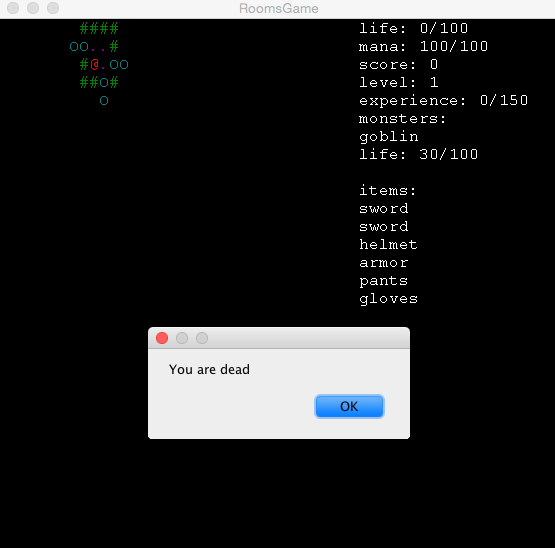
\includegraphics[width=\textwidth,height=\textheight,keepaspectratio]{./img/firstiterationui.png}
  \caption{Versión definitiva de la interfaz de usuario para el texto generado}
  \label{fig:firstiterationui}
\end{figure}

\subsubsection{Segunda idea: \textit{TextArea}}

Tras recibir el feedback decidimos cambiar la forma en la que mostramos al usuario estas frases por tres razones. La primera es que resulta desconcertante para el jugador vidente, dado que no es necesario para él o ella. Esto se podría solventar añadiendo una opción que se permita activar o desactivar esta opción, pero no es una solución óptima.
La segunda razón es que estos ``pop-ups'' no son un mecanismo de salida óptimo para las salidas rutinarias, como en nuestro caso, y rompe el ``flujo de trabajo''.
La tercera y última razón es que los usuarios invidentes no suelen usar elementos de este tipo, si no que están más acostumbrados a usar areas de texto donde se almacenan las últimas frases generadas.

En base a estas ideas decidimos crear el área de texto seleccionada, que permanecerá abierta siempre y cuando el jugador no decida cerrarla (permitiendo a los usuarios videntes no usarla). Una vez que algo suceda en el juego que requiera que se genere una descripción, dicha descripción será enviada al área de texto, el ``foco'' de las aplicaciones cambiará para que se sitúa en esa área de texto y el lector de pantalla que usemos leerá dicha descripción. Para que el ``foco'' vuelva a situarse en el juego, deberemos de pulsar cualquier tecla.
De esta forma solucionamos todos los inconvenientes que los ``pop-ups'' causaban a los usuarios y mejoramos la interfaz gráfica y accesibilidad del proyecto.

En ~\ref{lastiterationui} se puede encontrar una captura de pantalla donde se muestra el estado final de la parte de la interfaz de usuario que muestra las frases generadas.

\begin{figure}
    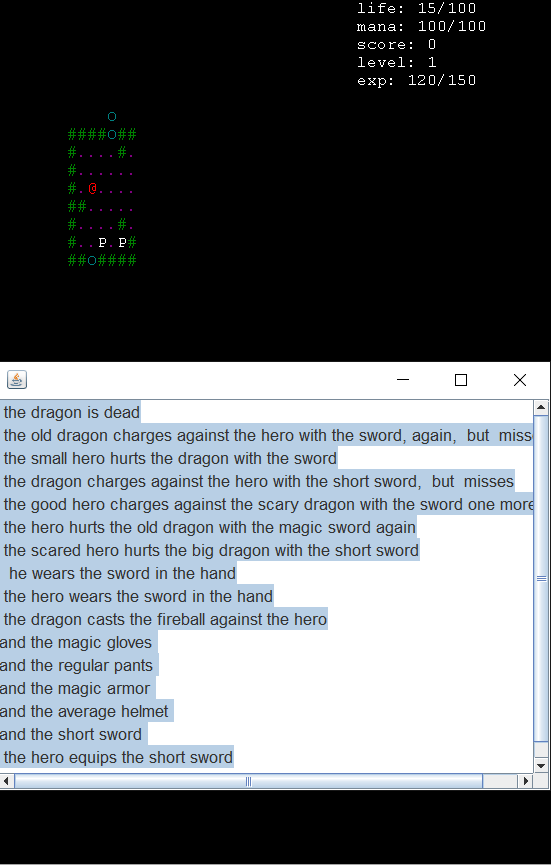
\includegraphics[width=\textwidth,height=\textheight,keepaspectratio]{./img/lastiterationui.png}
  \caption{Versión definitiva de la interfaz de usuario para el texto generado}
  \label{fig:lastiterationui}
\end{figure}

\subsection{Generación aleatoria de mapas y elementos}

La generación aleatoria de mapas y elementos dentro del mismo es muy importante en un juego de género \textit{roguelike}. A continuación explicaremos las decisiones tomadas en base a este tema.

\subsubsection{Primera idea: Generación completamente aleatoria}

En un primer momento nuestra decisión fue la de generar todo de manera aleatoria, sin considerar ningún aspecto externo, pero manteniendo la generalidad en el código para poder cambiar su comportamiento en cualquier momento. Esto causaba que algunas mazmorras fueran muy complicadas cuando el jugador todavía no tenía el equipamiento necesario para enfrentarse a dichos enemigos o demasiado sencilla en otros momentos.

Este problema fue mencionado la primera vez que recibimos feedback y por ello decidimos cambiarlo por algo un poco más complejo. En el mundo del rol, tener en cuenta ciertas características del usuario para generar elementos externos se denomina \textit{generación de encuentros}, que es lo que tuvimos en cuenta.

\subsubsection{Segunda idea: Generador de encuentros}
\label{generadorencuentros}

En vez de generar mapas, enemigos y elementos de manera completamente aleatoria, podemos generarlos en base al nivel que tienen ciertos personajes. Si el personaje que controla el usuario tiene nivel 10, entonces los enemigos que se encuentran deben de ser de un nivel, por ejemplo, entre 8 y 12, mientras que los elementos que los enemigos sueltan al morir (como las espadas y armaduras) también deben de tener un nivel similar para que la progresión tenga sentido y eliminar enemigos tenga un cierto nivel de recompensa.

De esta forma podremos, en base al nivel dado, podremos generar enemigos con diferentes características que se adapten a lo que necesitamos:

\begin{lstlisting}[language=java]
Rat rat = new Rat(this.getMap(), this, position, new ArrayList<String>(), level);
\end{lstlisting}

\subsection{Comportamiento de los enemigos}

\begin{figure}
    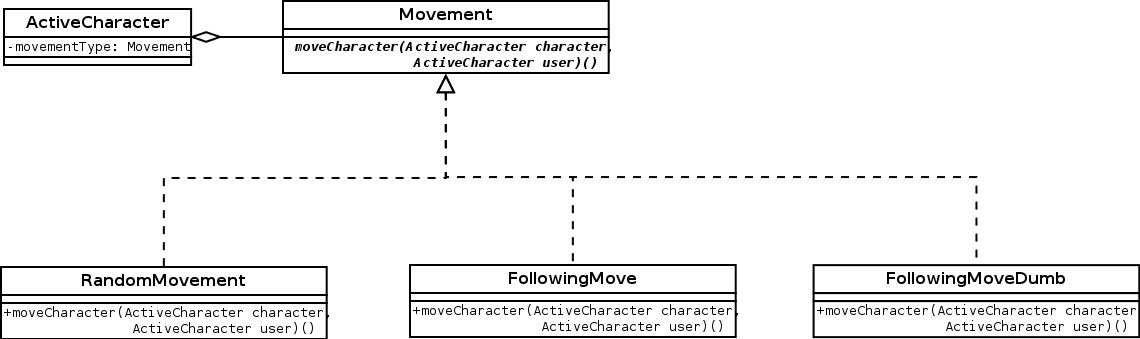
\includegraphics[width=\textwidth,height=\textheight,keepaspectratio]{./img/iaenemy.png}
  \caption{Diagrama de clases sobre el comportamiento de los enemigos}
  \label{fig:iaenemy}
\end{figure}